\chapter{Inleiding} 

\label{chap:inleiding} In deze thesis, die kadert binnen het Unipept-project,
wordt de mogelijkheid onderzocht om een metagenomics probleem om te zetten in
een metaproteomics probleem. Voor we iets meer vertellen over de structuur en de
opbouw van deze thesis is het belangrijk de titel van de thesis te
verduidelijken. Metagenomics en metaproteomics zijn namelijk twee termen uit de
biologie die wel wat uitleg vergen. In deze inleiding leggen we uit wat beide
termen inhouden, bekijken we de onderliggende concepten, lichten we toe wat
Unipept precies is en welke rol Unipept zal spelen in dit onderzoek.

\section{Genomics en proteomics}

Genomics is de studie waarbij genomen worden onderzocht. Een genoom is het
geheel van de genetische samenstelling van het materiaal in een organisme en
wordt uitgedrukt als een DNA-sequentie, bestaande uit nucleotiden. Er kunnen
verschillende analyses uitgevoerd worden op een genoom, maar voor alle
experimenten zal het genoom eerst moeten worden gesequeneerd om de ordering van
de DNA-baseparen te bepalen. Dat proces heeft een heel aantal korte
DNA-fragmenten (DNA-reads genaamd) als resultaat, zoals in \Vref{fig:genomics}
wordt geïllustreerd. Die verzameling van korte reads dient als basis voor een
aantal processen: \textit{i)} assembly, waarbij de korte reads allemaal samen
tot één consensusgenoom worden samengevoegd en \textit{ii)} mapping, waarbij de
reads op andere genomen worden gemapt om zo de afstand (verwantschap) van het
genoom in kwestie tot andere genomen te bepalen. Bij die laatste stap wordt
gebruikt gemaakt van genoomdatabanken waarin alle gekende genomen zijn
opgeslagen. Voorbeelden van genoomdatabanken zijn INSDC en RefSeq. Een recente
read mapper is bijvoorbeeld ALFALFA\cite{vyverman2015long}.

\begin{figure}
	\centering
	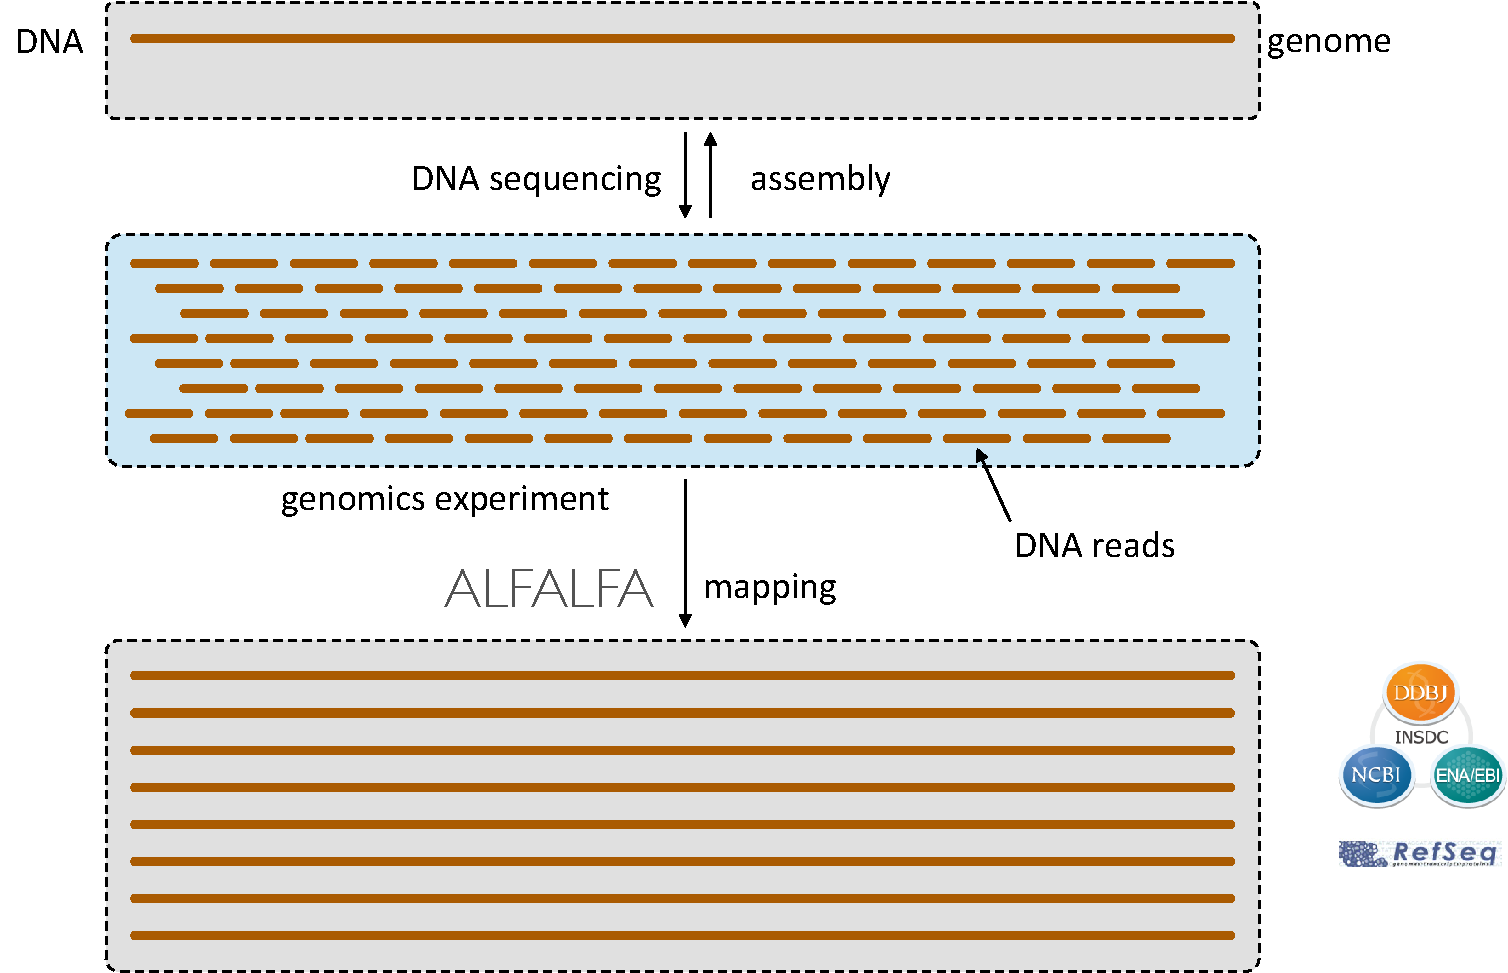
\includegraphics[width=0.8\textwidth]{includes/genomics}
	\caption{Illustratie van een genomics experiment. Een genoom, voorgesteld 
	door een bruine lijn, wordt gesequeneerd in verschillende DNA reads. Deze 
	reads kunnen dan opnieuw worden geassembleerd naar een volledig 
	consensusgenoom of kunnen worden gemapt op meerdere genomen aan de hand van 
	DNA read 
	mappers en genoomdatabanken.}
	\label{fig:genomics}
\end{figure}

Verwant aan het genoom is het proteoom. De studie van proteomen wordt proteomics
genoemd. Een proteoom bestaat uit de volledige set aan eiwitten die geëncodeerd
in door een genoom, een organisme of een deel ervan. Net als een genoom kan een
proteoom ook worden gesequeneerd in protein reads, peptiden genaamd. Die protein
reads kunnen dan net zoals DNA reads gemapt worden aan de hand van tools, zoals
Unipept\cites{mesuere2012unipept, mesuere2014unipept}, worden gemapt op
eiwitdatabanken, zoals geïllustreerd in \Vref{fig:proteomics}.
UniProt\cite{uniprot2014uniprot} is een voorbeeld van zo'n soort eiwitdatabank.

\begin{figure}
	\centering
	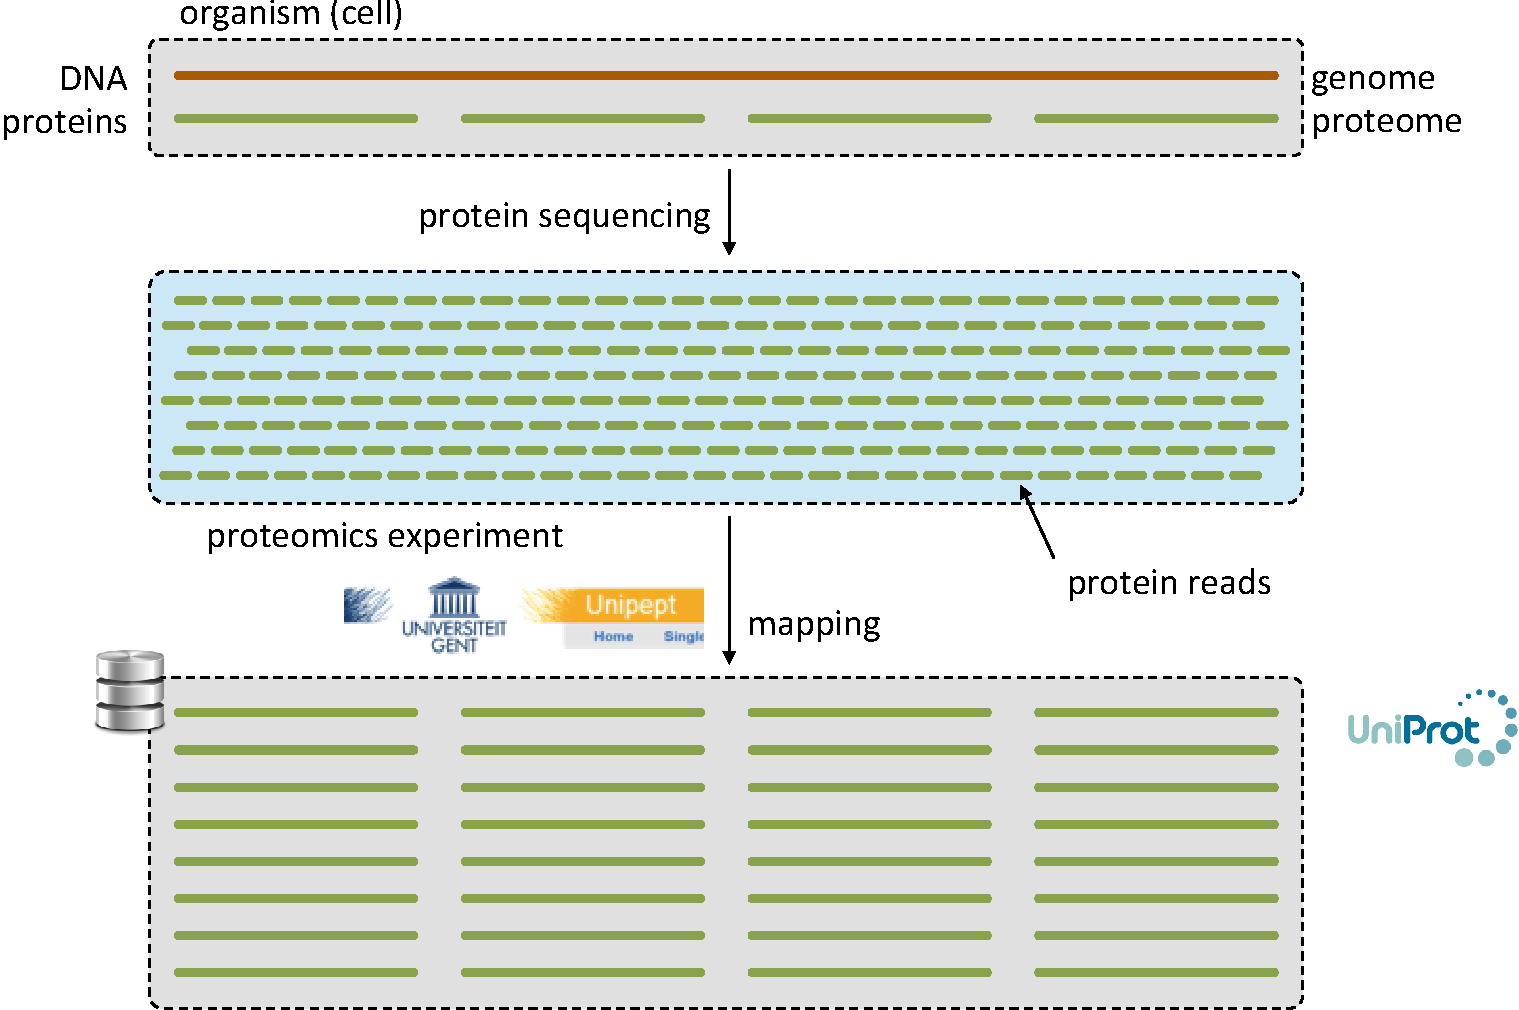
\includegraphics[width=0.8\textwidth]{includes/proteomics}
	\caption{Illustratie van een proteomics experiment. Eiwitten, geannoteerd 
	op een genoom, worden gesequeneerd in protein reads. Die reads kunnen dan 
	worden gemapt op overeenkomstige proteomen uit eiwitdatabanken.}
	\label{fig:proteomics}
\end{figure}

\section{Metagenomics en metaproteomics} 

Wanneer stalen worden genomen uit de natuur, bijvoorbeeld bij vijveronderzoek,
of in de medische wereld, bijvoorbeeld bij de analyse van iemands stoelgang,
krijgen onderzoekers te maken met gemeenschappen in plaats van geïsoleerde
specimen. Ze hebben met andere woorden te maken met stalen van meerdere genomes
of metagenomes en meerdere proteomes of metaproteomes. Daarbij komt ook nog eens
dat slechts één procent van de organismen die in de natuur wordt gevonden, in
een lab kan worden gekweekt. Het is dus belangrijk om rechtstreeks met stalen
uit de natuur te kunnen werken en voor een vlotte analyse van die stalen is het
noodzakelijk dat er technieken bestaan die meerdere genomen en proteomen
tegelijkertijd kunnen verwerken en analyseren. Wanneer we het hebben over het
analyseren van metagenomes en metaproteomes bevinden we ons respectievelijk in
het onderzoeksgebied van de metagenomics en de metaproteomics.

Bij dit soort onderzoek zijn er drie grote vragen: \textit{i)} Welke organismen
bevinden zich in een staal? \textit{ii)} Wat doen ze precies? en \textit{iii)}
Hoe doen ze het? In deze thesis houden we ons vooral bezig met de eerste vraag.

Onderzoek in metagenomics gebeurt typisch op twee manieren. De eerste manier is
\emph{targeted metagenomics} waarbij een specifiek stuk, meestal een deel van
het 16S ribosomaal RNA, uit de verschillende organismen in het staal worden
gesequeneerd. Een tweede manier is \emph{shotgun metagenomics} waarbij de
volledige DNA strands uit het metagenoom worden gesequeneerd. Opnieuw aan de
hand van verschillende genoomdatabanken kan de mapping van die reads naar
gesequeneerde genomen gebeuren. Beide aanpakken zijn geïllustreerd in
\Vref{fig:metagenomics}.

\begin{figure}
	\centering
	\begin{subfigure}{0.49\textwidth}
		\centering
		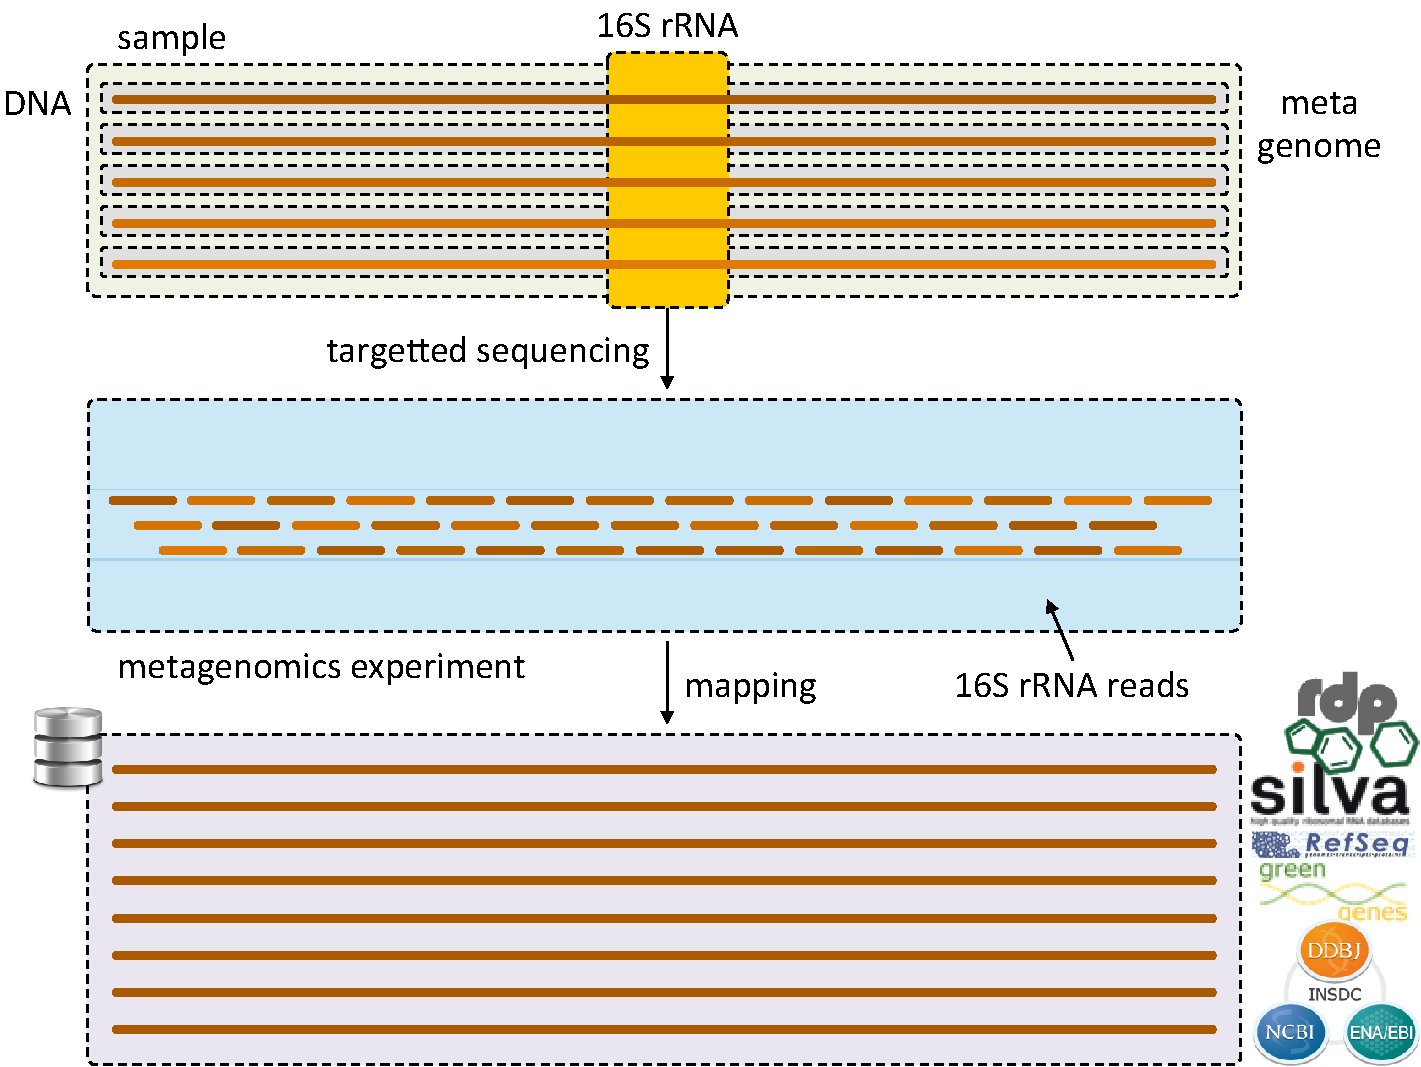
\includegraphics[width=\textwidth]{includes/targetted_metagenomics}
		\caption{}
	\end{subfigure}
	\begin{subfigure}{0.49\textwidth}
		\centering
		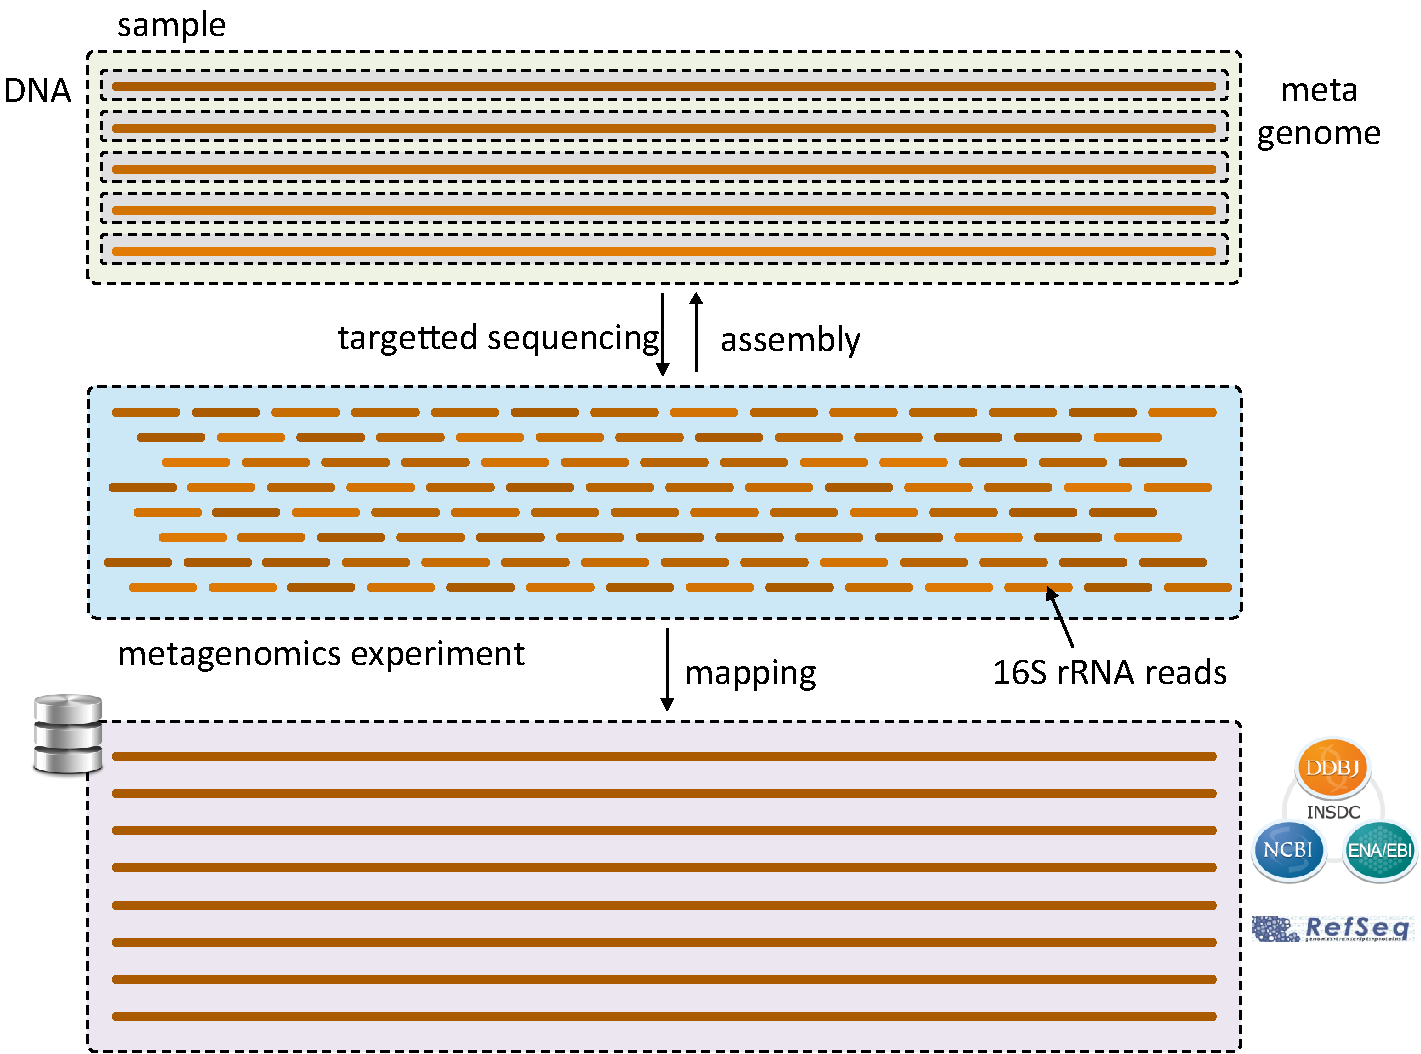
\includegraphics[width=\textwidth]{includes/shotgun_metagenomics}
		\caption{}
	\end{subfigure}
	
	\caption{Illustratie van een metagenomics experiment. Links de 16S rRNA 
	variant, rechts de shotgun variant. Bij een metagenomics experiment wordt 
	(een gedeelte van) de DNA strands uit een metagenoom gesequeneerd en daarna 
	op genoomdatabanken gemapt.}
	\label{fig:metagenomics}
\end{figure}

Het proces van metagenomics kan, analoog aan de processen van genomics en 
proteomics, toegepast worden op metaproteomics. Dat wordt geïllustreerd in 
\Vref{fig:metaproteomics}. Hierbij worden alle eiwitten op de DNA strands uit 
het sample geannoteerd en gesequeneerd in protein reads of peptiden. Die 
peptiden kunnen vervolgens opnieuw, bijvoorbeeld door Unipept, worden gemapt op 
eiwitdatabanken.

\begin{figure}
	\centering 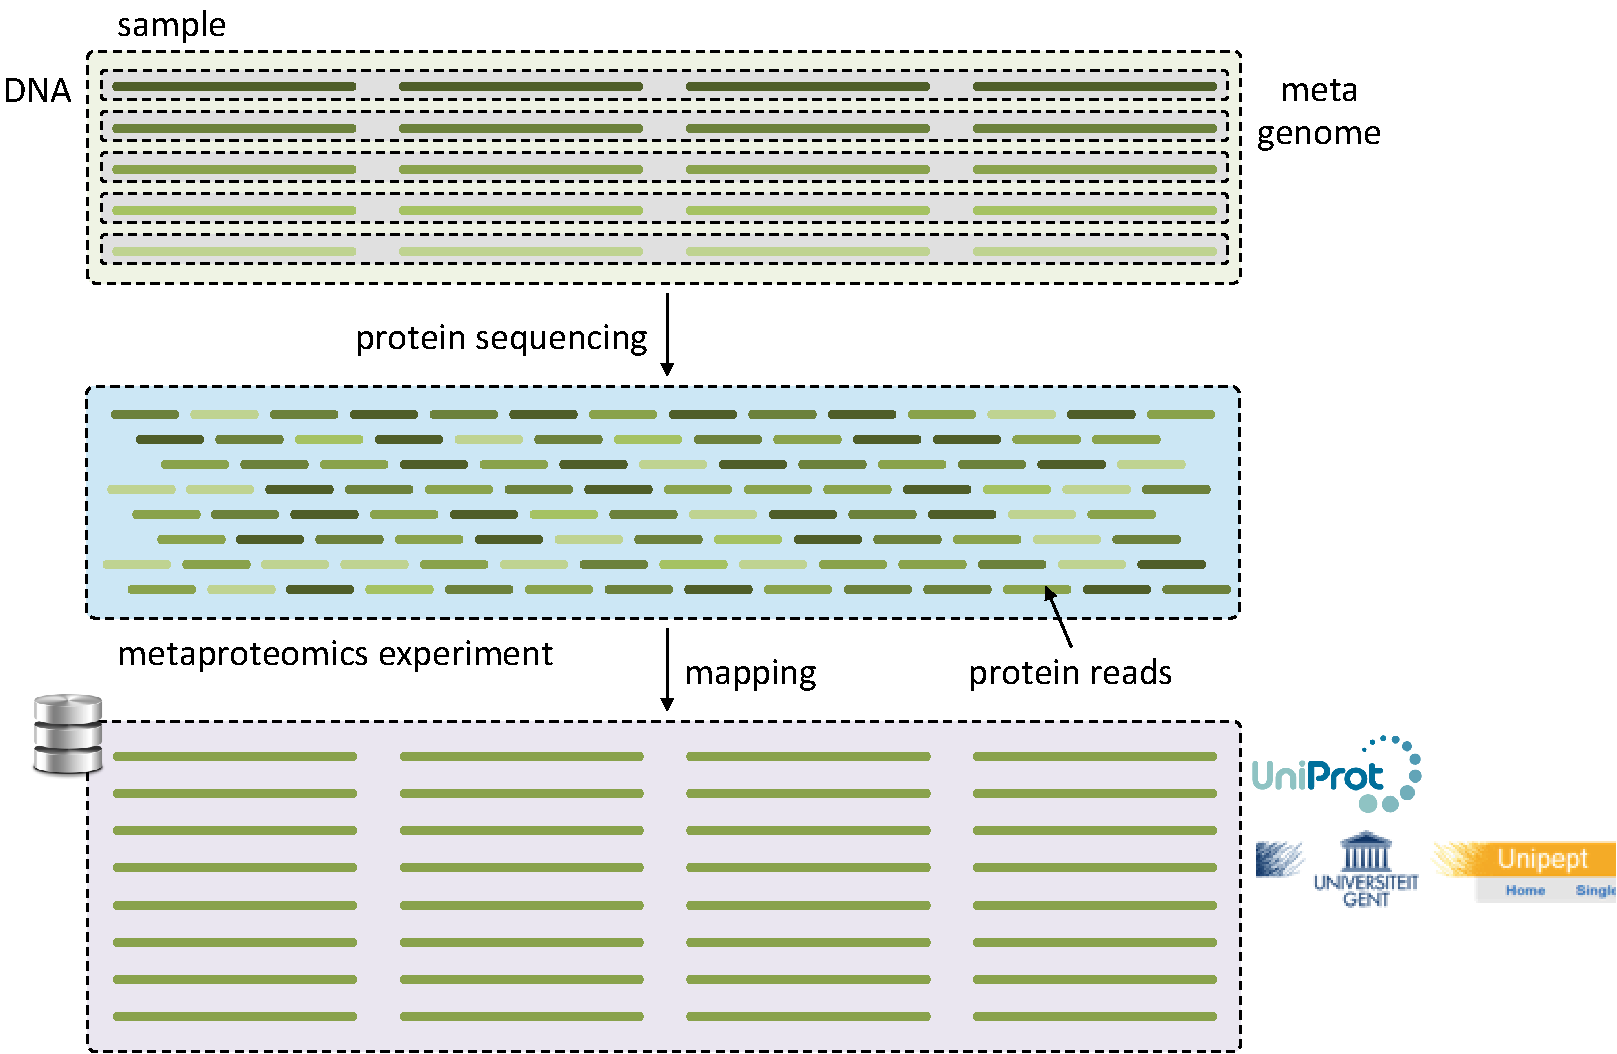
\includegraphics[width=0.8\textwidth]{includes/metaproteomics}
	\caption{Illustratie van een metaproteomics experiment. Alle eiwitten,
	geannoteerd op de verschillende DNA strands, worden gesequeneerd in
	protein reads, peptiden genaamd. Die peptiden kunnen dan worden gemapt op
	overeenkomstige proteomen aan de hand van eiwitdatabanken.}
	\label{fig:metaproteomics}
\end{figure}

\section{Van metagenoom naar metaproteoom}
De klassieke oplossing voor de mapping van een reeks DNA reads op genomen in een
genoomdatabank is het gebruik van BLAST, of verwante tools. Die tools zijn vaak
zeer traag en vereisen zeer veel rekencapaciteit.  Aangezien Unipept
al in staat is om zeer snel metaproteomen te analyseren zou het erg voordelig
zijn om dat metagenomics probleem om te zetten naar een metaproteomics probleem.
Dat is dan ook wat we proberen te doen. Het grootste voordeel van die omzetting
is dat we voor de meeste stappen integraal gebruik kunnen maken van de Unipept
Metaproteomics Analyse Pipeline. Die pipeline is al geïmplementeerd en 
geoptimaliseerd om alles in zo weinig mogelijk tijd te berekenen. Wat dan 
nog rest is de conversie van en naar metagenomics.

De omzetting zelf gebeurt volgens de werkwijze aangegeven in
\Vref{fig:van_naar}. Voor elke DNA read in een metagenomics dataset kunnen we
een proteomics experiment doen. Hierbij zoeken we, bijvoorbeeld aan de hand van
FragGeneScan, alle (fragmenten van) eiwitten in de DNA read in kwestie. De
bekomen eiwitten worden opgedeeld in tryptische peptiden, waarna elke peptide
afzonderlijk op zijn taxonomische identificatie wordt gemapped door middel van
het lowest common ancenstor (LCA) algoritme. Aan de hand van een uitbreiding van
dit lowest common ancestor algoritme kunnen we de bekomen taxa aggregeren naar
een consensusclassificatie. Dat proces zullen we vanaf nu aanduiden met de
Unipept Metagenomics Analysis Pipeline, of ook wel UMAP.

\begin{figure}[hbt]
	\centering 
	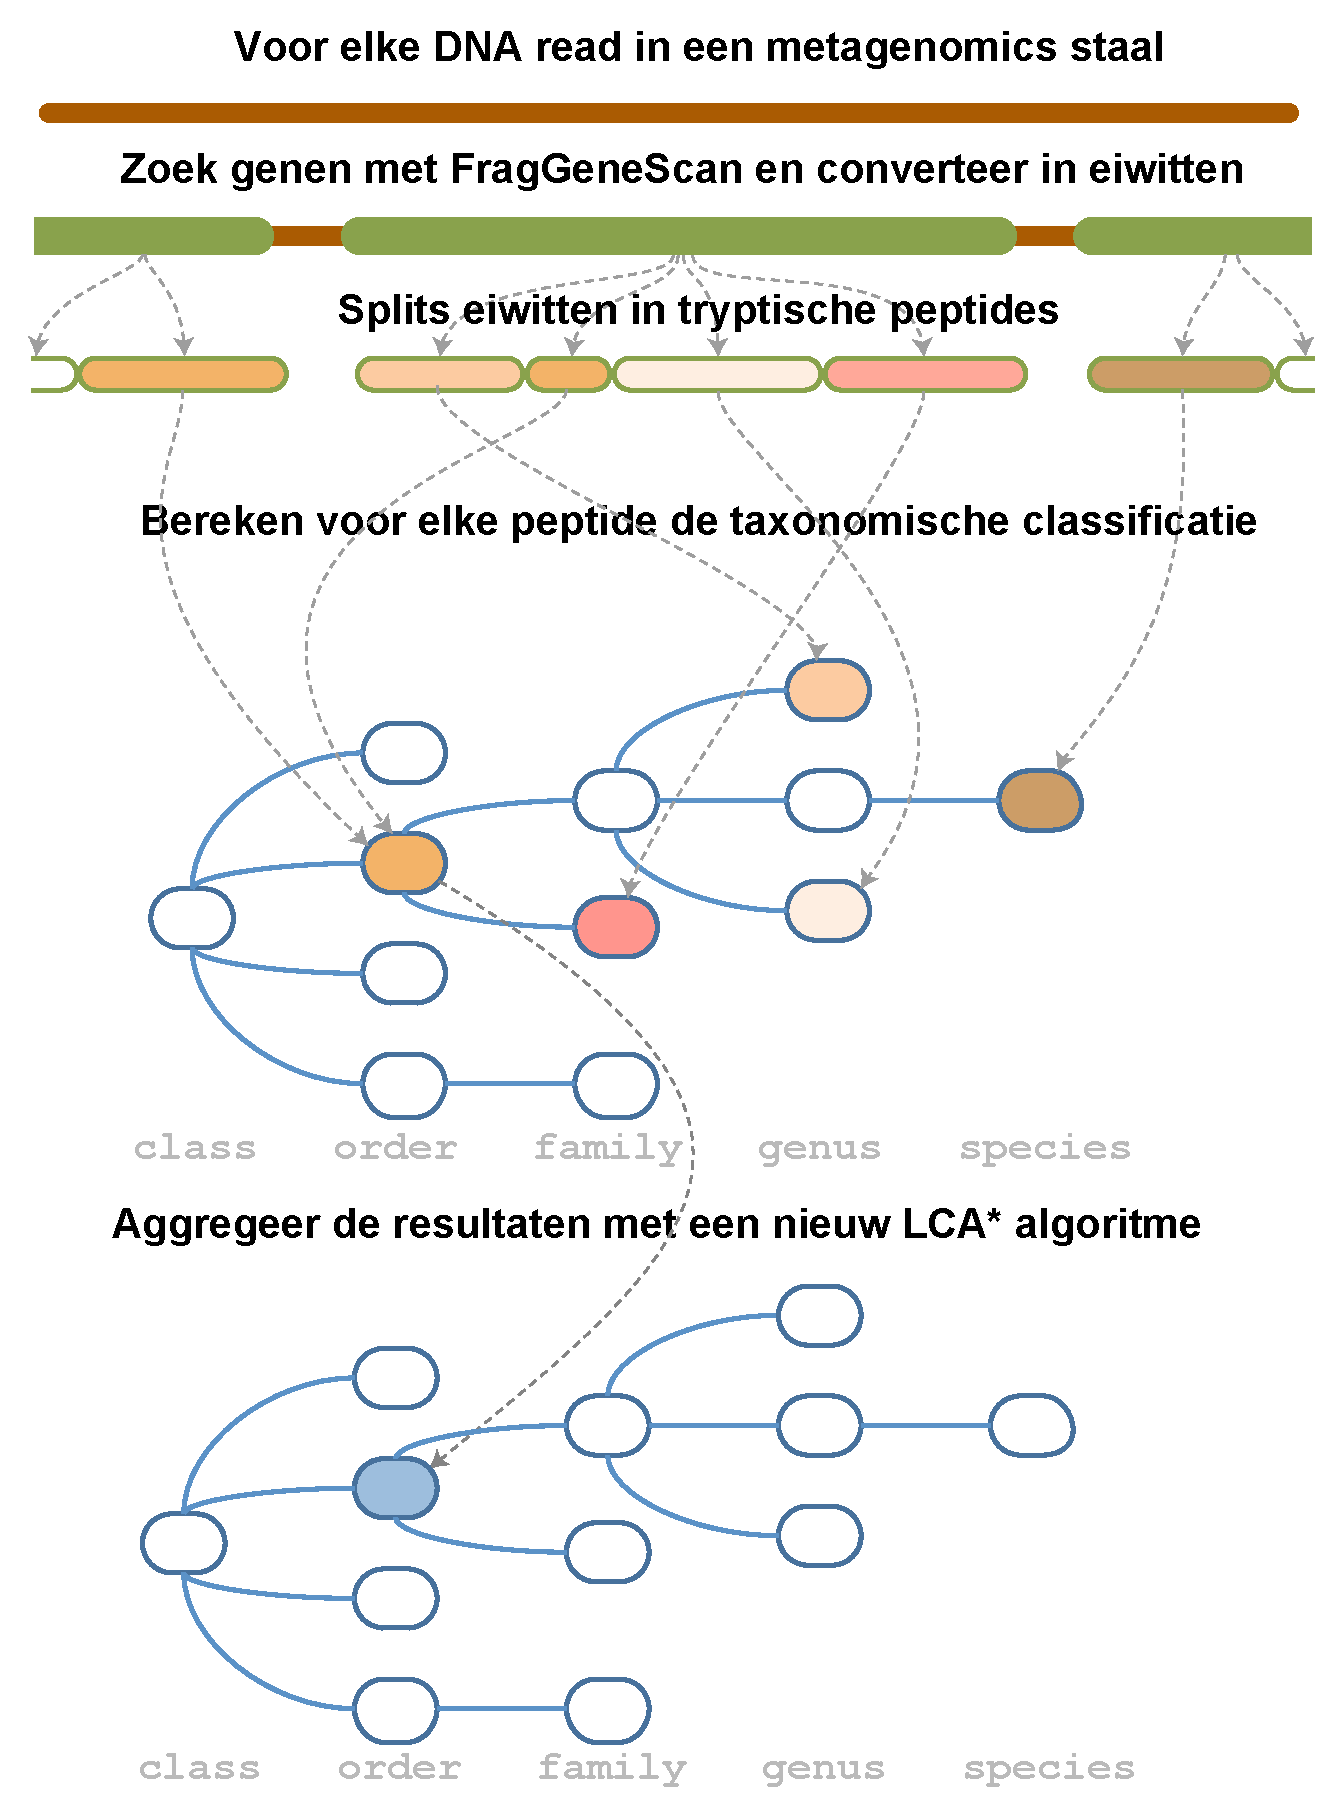
\includegraphics[width=0.6\textwidth]{includes/van_metagenoom_naar_metaproteoom}
	\caption{Illustratie van de werkwijze om een metagenomics probleem om te 
	zetten naar een metaproteomics probleem. Voor elke DNA read in het 
	metagenomics sample kunnen we een proteomics experiment doen. Hierbij 
	zoeken we, bijvoorbeeld aan de hand van FragGeneScan, alle eiwitten op 
	de DNA read in kwestie. De bekomen eiwitten worden opgedeeld in 
	tryptische peptiden waarna elke peptide afzonderlijk op zijn taxonomische 
	identificatie wordt gemapped door middel van het lowest common ancestor 
	(LCA) algoritme. Aan de hand van een uitbreiding van dit lowest common 
	ancestor algoritme kunnen we de bekomen taxa aggregeren naar een 
	consensusclassificatie.}
	\label{fig:van_naar}
\end{figure}

In \Vref{chap:lca*} bespreken we de motivatie en implementatie van het nieuwe 
LCA* algoritme gebruikt in de laatste stap, waarna we in \Vref{chap:casestudy} 
de performantie benchmarken van de nieuwe Unipept Metagenomics Analysis 
Pipeline.

\section{Unipept}
In dit hoofdstuk is de naam Unipept een aantal keer gevallen. Aangezien deze
thesis kadert binnen het Unipept-project wordt in deze sectie een korte
beschrijving van Unipept gegeven en wordt uitgelegd waar Unipept zich momenteel
bevindt in de bovenstaande processen.

Kort samengevat is Unipept een framework met een gebruiksvriendelijke
webinterface om de biodiversiteit van grote en complexe metaproteomics samples
te onderzoeken aan de hand van informatie uit tryptische peptiden. Achter de
webinterface bevindt zich een indexstructuur die ervoor gemaakt is om snel alle
eiwitten uit de UniProtKB op te vragen waar de tryptische peptide in voorkomt.
Door het gebruik van een speciale lowest common ancestor aanpak kan ook de
taxonomische identificatie aan een peptide gekoppeld worden die bestand is tegen
verkeerde identificaties, classificaties en onjuistheden in de taxonomieboom.
Die achterliggende indexstructuur is naast de webinterface ook aanspreekbaar
via de Unipept command-line interface (CLI) die een interface aanbiedt voor de 
Unipept web services. De CLI laat de gebruiker toe grote datasets te verwerken 
zonder dat via de browser te moeten doen.

\Vref{chap:cli} geeft na een inleiding tot de Unipept command-line interface een
reeks van problemen met bijhorende oplossingen die naar boven zijn gekomen
tijdens het intensief gebruik van de tools. In \Vref{chap:vis} geven we een
overzicht van de al bestaande visualisaties in Unipept. Daarnaast motiveren we
de abstractie en modularisatie van die visualisaties in een apart Unipept
visualisation framework.

\section{Geschreven code}

Alle code geschreven binnen de context van deze thesis is verzameld op de UGent
GitHub onder de Unipept organisatie en voornamelijk onder de repositories
\texttt{unipept-visualizations} en \texttt{unipept-metagenomics-scripts}.
Toegang tot deze repositories kan gegeven worden door de promotor of begeleider
van deze thesis.